\chapter{Método de trabajo y herramientas}
\label{chap:metodo}

\drop{E}{n} este capitulo se expone la metodología seguida para llevar a cabo el proyecto y se
justifica por qué se considera el método más satisfactorio a la hora de implementar este
\acs{TFG}. Además, se seleccionan y nombran las diferentes herramientas utilizadas para el
desarrollo del mismo tanto software como hardware.

\section{Metodología de trabajo}

Al comenzar este \acs{TFG} sólo disponíamos de una idea general del sistema que queríamos
desarrollar. Puesto que los requisitos de los que disponíamos no eran detallados, se decidió optar
por un modelo de desarrollo evolutivo para ir detallando las especificaciones a lo largo del
progreso del proyecto. En particular, el de prototipos desechables o prototipado evolutivo.

El desarrollo evolutivo se basa en la idea de desarrollar una implementación inicial, exponiéndola a
los comentarios del usuario y refinándola a través de las diferentes versiones hasta que se
desarrolla un sistema adecuado~\cite{Sommerville14}.

En la Figura~\ref{fig:modelo-evolutivo} se muestra el diagrama de flujo seguido por un modelo
evolutivo en el que se puede ver como las actividades de especificación, desarrollo y validación se
realizan de forma concurrente con una rápida retroalimentación entre ellas.

\begin{figure}[!h]
  \begin{center}
    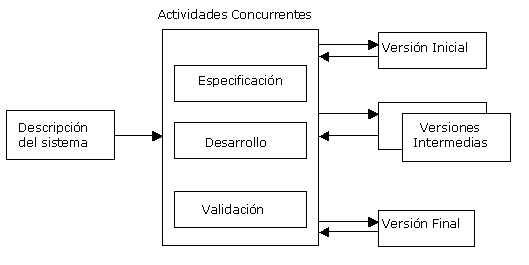
\includegraphics[width=0.75\textwidth]{/modelo-evolutivo.jpg}
    \caption{Diagrama de flujo del modelo de desarrollo evolutivo}
    \label{fig:modelo-evolutivo}
  \end{center}
\end{figure}

\subsection{Prototipado evolutivo}

El prototipado evolutivo es un modelo de desarrollo de software basado en la realización de
prototipos funcionales hasta llegar a un producto final. Se parte de los requisitos mejor
comprendidos y con mayor prioridad, y se van definiendo los detalles conforme avanza el desarrollo
de las diferentes versiones.

Un cliente, a menudo, define un conjunto de objetivos generales para el software, pero no identifica
los requisitos detallados de entrada, proceso o salida. De igual forma, el responsable del
desarrollo del software puede no estar seguro de la eficacia de un algoritmo o de la forma en que
debería plantearse la \acs{IPO}. En estas y otras muchas situaciones, un paradigma de construcción
de prototipos puede ofrecer el mejor enfoque~\cite{Pressman10}.

El esquema general de prototipado evolutivo se puede ver en la Figura ~\ref{fig:prototipo}. El
paradigma comienza con una recolección de requisitos, es decir, el desarrollador y el cliente
definen los objetivos globales para el software, identifican los requisitos conocidos y las áreas
donde se necesita más definición. Entonces aparece un diseño rápido centrado en los aspectos que
serán visibles para el cliente y se construye un prototipo. Este prototipo es evaluado por el
cliente y se utiliza para refinar los requisitos del software. Esta iteración se repite hasta llegar
al resultado final.

\begin{figure}[!h]
  \begin{center}
    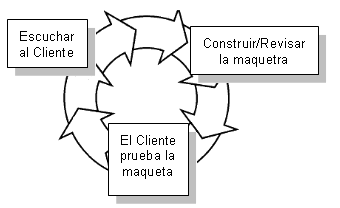
\includegraphics[width=0.6\textwidth]{/prototipo.png}
    \caption{Paradigma de construcción de prototipos}
    \label{fig:prototipo}
  \end{center}
\end{figure}

Entre las ventajas del uso del prototipado evolutivo hay que destacar:

\begin{itemize}
  \item La continua obtención de prototipos permite al cliente observar y dirigir el desarrollo del
    software.
  \item Las funcionalidades más importantes son desarrolladas en las primeras fases del proyecto y,
    por tanto, son las funcionalidades que más veces se ha probado su correcto funcionamiento.
  \item Como se evalúan prototipos intermedios, es más fácil comprobar si los requisitos planteados
    son correctos y viables.
\end{itemize}

Por otro lado, el prototipado evolutivo  también puede presentar algunas desventajas:

\begin{itemize}
  \item Resulta difícil estimar el coste final del proyecto debido al desconocimiento del número de
    iteraciones a realizar.
  \item Resulta muy difícil y costoso realizar cambios en la arquitectura del software.
\end{itemize}

Debido a estos problemas, aplicar el prototipado evolutivo resulta muy complejo para grandes
proyectos pero resulta conveniente utilizarlo en sistemas pequeños y de tamaño medio como el planteado en este \acs{TFG}.

\section{Herramientas}

\subsection{Hardware}
\begin{definitionlist}
  \item[]
\end{definitionlist}

\subsection{Software}

% Local Variables:
% TeX-master: "main.tex"
%  coding: utf-8
%  mode: latex
%  mode: flyspell
%  ispell-local-dictionary: "castellano8"
% End:
